% Created 2015-08-17 Mon 21:40
\documentclass[presentation]{beamer}
\usepackage[utf8]{inputenc}
\usepackage[T1]{fontenc}
\usepackage{fixltx2e}
\usepackage{graphicx}
\usepackage{longtable}
\usepackage{float}
\usepackage{wrapfig}
\usepackage{rotating}
\usepackage[normalem]{ulem}
\usepackage{amsmath}
\usepackage{textcomp}
\usepackage{marvosym}
\usepackage{wasysym}
\usepackage{amssymb}
\usepackage{hyperref}
\tolerance=1000
\usepackage{minted}
\usepackage{multirow}
\usepackage{minted}
\usepackage{fontspec}
\usepackage{graphicx}
\usepackage{subcaption}
\newminted{ruby}{fontsize=\scriptsize}
\usepackage{./theme/beamerthemeCristian}
\usepackage[nocolor]{./theme/beamerAlvinMacros}
\usepackage[absolute,overlay]{textpos}
\setlength{\TPHorizModule}{\paperwidth}
\setlength{\TPVertModule}{\paperheight}
\textblockorigin{0mm}{0mm}
\usepackage{natbib}
\usepackage{bibentry}
\usepackage{dirtree}
\newcommand\Fontvi{\fontsize{6}{7.2}\selectfont}
\nobibliography*
\usetheme{default}
\usecolortheme{}
\usefonttheme{}
\useinnertheme{}
\useoutertheme{}
\author{\\ \vspace{0.5cm} Cristian Ruiz, Emmanuel Jeanvoine and Lucas Nussbaum \\ \vspace{0.5cm} INRIA Nancy, France \\ \vspace{0.5cm} VHPC'15}
\date{}
\title{Performance Evaluation of Containers for HPC}
\hypersetup{
  pdfkeywords={},
  pdfsubject={},
  pdfcreator={Emacs 24.3.1 (Org mode 8.2.10)}}
\begin{document}




\sloppy
\frame{
  \thispagestyle{empty}
  \titlepage
  \begin{center}
    
\includegraphics[height=1.2cm]{logos/inr_logo_sans_sign_coul.png}
    \hspace{0.5cm}
  \insertlogo{
\includegraphics[height=1.2cm]{logos/grid5000.png}}
   \hspace{0.5cm}
  \insertlogo{
\includegraphics[height=1.2cm]{logos/logo_loria_complet_couleur.pdf}}
  \end{center}

}

\tableofcontents



\section{Introduction}
\label{sec-1}

{\setbeamercolor{background canvas}{bg=basicallyblack}
\usebeamercolor[fg]{inverted text}
\begin{frame}[label=sec-1-1]{Linux Containers}


\par {\usebeamerfont{title} Container based virtualization}\par
\vspace{1cm} %\hfill
\end{frame}
}


\begin{frame}[label=sec-1-2]{Containers}
\begin{itemize}
\item \alert{Containers} refers generally to \alert{Operating-system-level virtualization},
where the \alert{kernel} of an operating system allows for multiple isolated \alert{user-space instances}.
\end{itemize}

\begin{figure}[!h]
  \center
  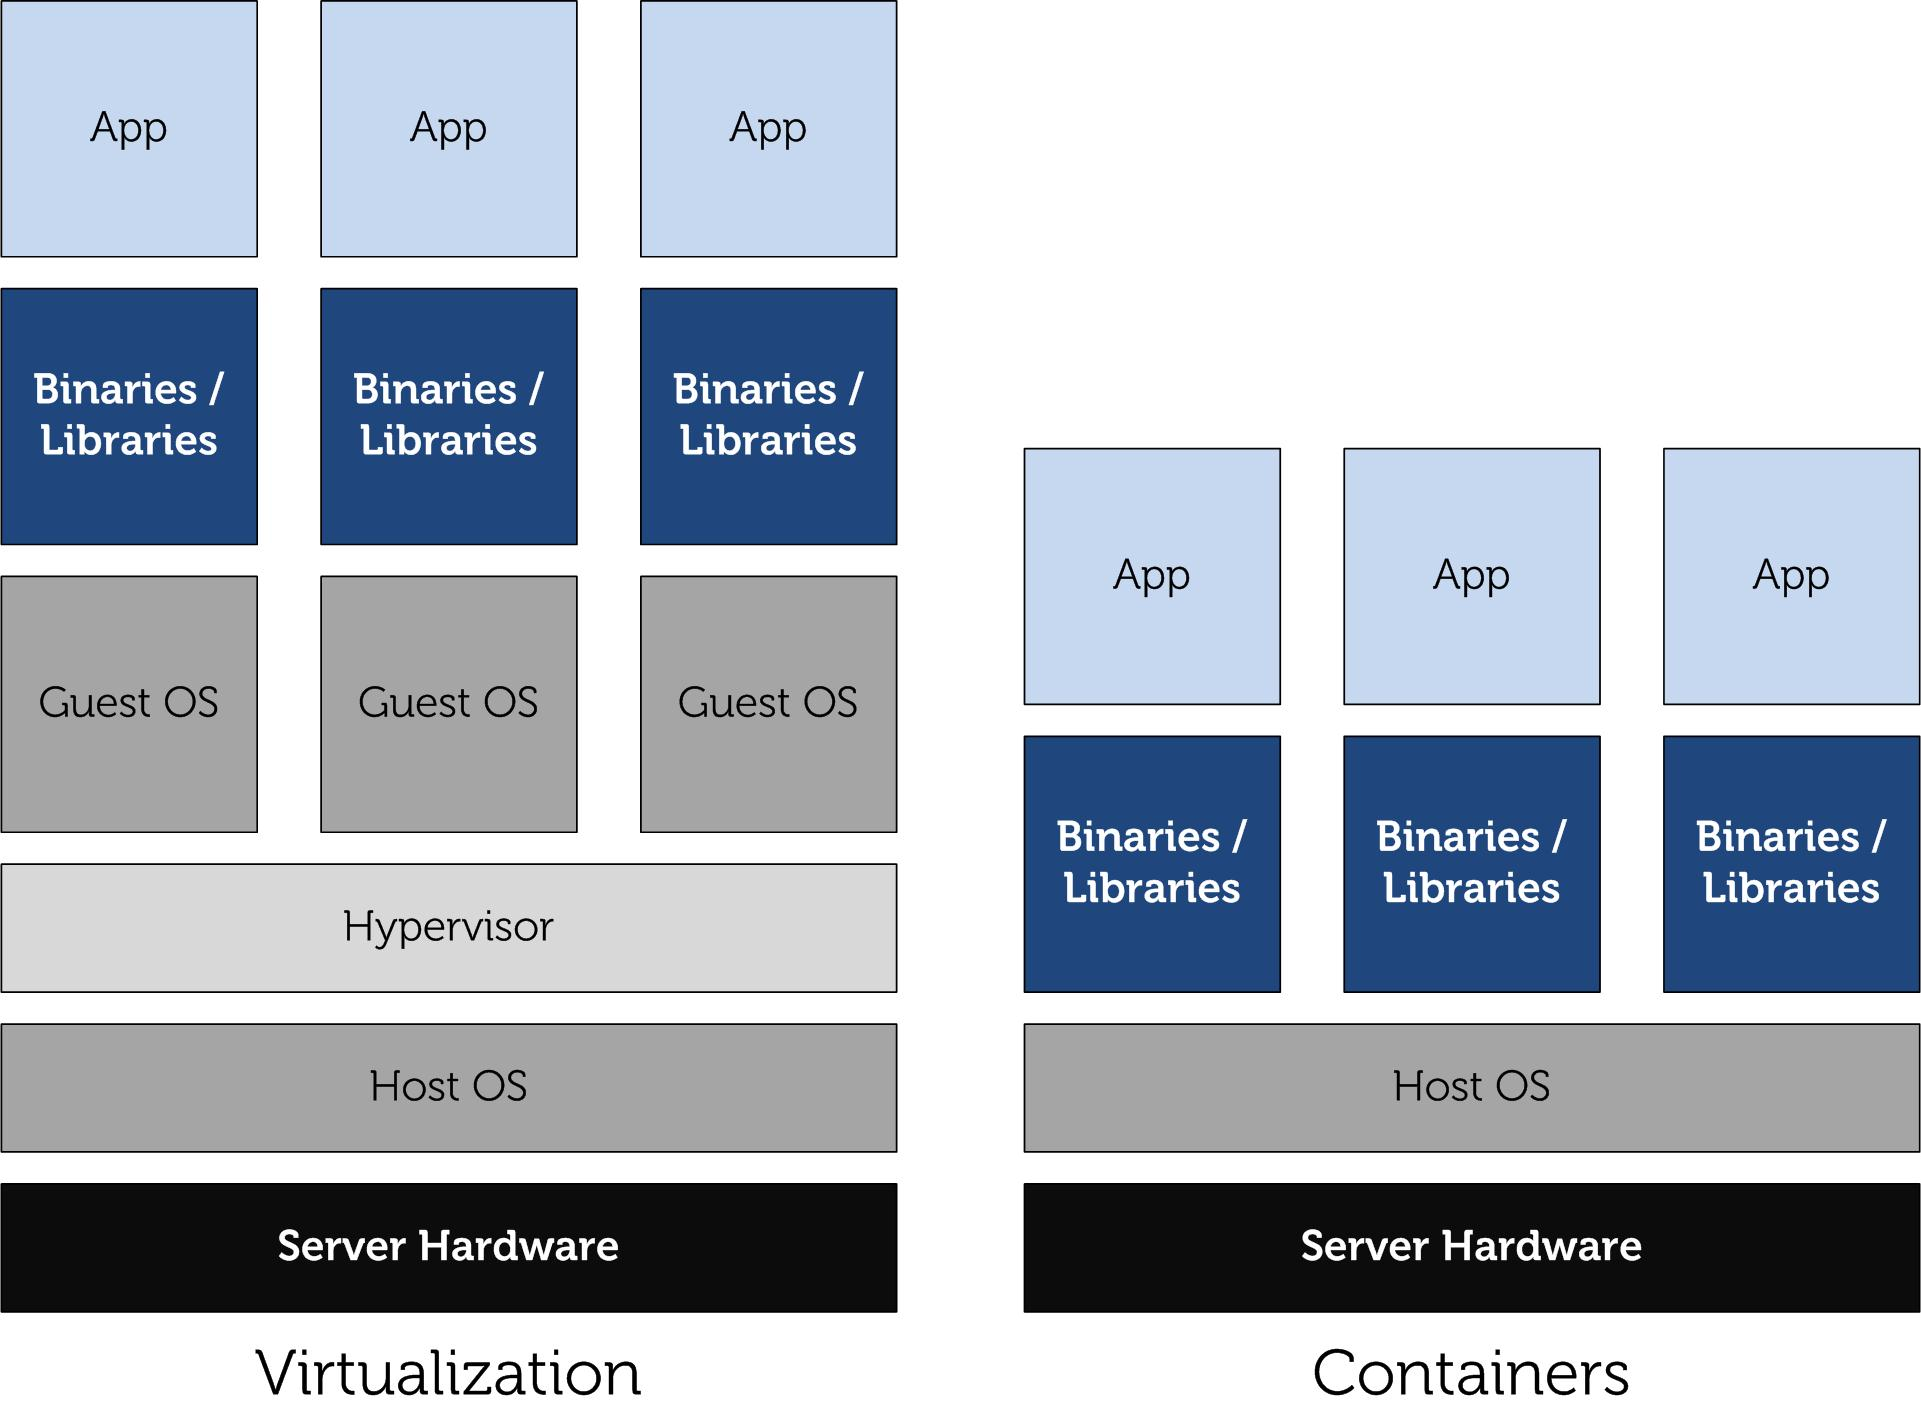
\includegraphics[scale=0.65]{figures/lxc-vm.jpg}
  \label{fig:hpc}
\end{figure}
\end{frame}

\begin{frame}[label=sec-1-3]{Implementations}
\begin{itemize}
\item Chroot
\item Linux-VServer
\item FreeBSD Jails
\item Solaris Containers
\item OpenVZ
\item Linux-Containers (LXC)
\end{itemize}
\end{frame}

\begin{frame}[label=sec-1-4]{\emph{namesapces and cgroups}}
\begin{itemize}
\item Both features incorporated in Linux kernel since 2006 (Linux 2.6.24).
\item Several container solutions: LXC, Docker, libcontainer, systemd-nspawn.
\end{itemize}

\begin{figure}[!h]
  \center
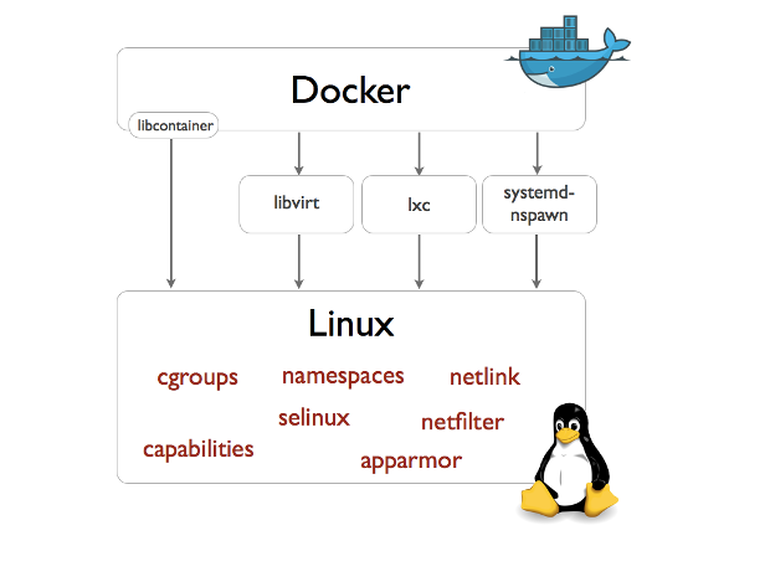
\includegraphics[scale=0.30]{figures/libcontainer-diagram.pdf}
  \label{fig:hpc}
\end{figure}
\end{frame}



\section{State of the art}
\label{sec-2}
\begin{frame}[label=sec-2-1]{Virtualization solutions for HPC}
\begin{itemize}
\item Youssef et al\cite{Youseff:2006:EPI:1308175.1308346} evaluated Xen using HPC
Challenge benchmarks and LLNL ASC Purple benchmarks.

\item Nussbaum et al\cite{nussbaum2009linux} compared Xen and KVM using
micro-benchmarks and the HPC Challenge benchmarks.

\item Regola et al\cite{regola2010recommendations} focuses on the I/O
performance of Xen, KVM and OpenVZ.

\item Public Cloud platforms: Amazon EC2 \cite{5353067} and Microsoft Azure\cite{Tudoran:2012:PEA:2168697.2168701}
  have been evaluated using Intel MPI benchmarks and scientific applications.
\end{itemize}
\end{frame}

\begin{frame}[label=sec-2-2]{Container performance evaluation}
\begin{itemize}
\item Matthews et al\cite{matthews2007quantifying} compared the performance of VMWare,
Xen, Solaris containers and OpenVZ using custom benchmarks.
\item Felter et al\cite{ibmtrdocker} evaluated the I/O performance of Docker using MySQL,
Linpack, Stream, RandomAccess, nuttcp, netperf, fio, and Redis.
\item Walter et al\cite{4482796} compared VMWare Server, Xen and OpenVZ using NetPerf, IOZone, and the NAS Parallel Benchmarks.

\item Xavier et al\cite{6498558} compared Linux VServer, OpenVZ,
LXC and Xen using the HPC Challenge benchmarks and the NAS
Parallel Benchmarks.
\end{itemize}
\end{frame}

{\setbeamercolor{background canvas}{bg=basicallyblack}
\usebeamercolor[fg]{inverted text}
\begin{frame}[label=sec-2-3]{In this work, we answer:}



\begin{itemize}
\item What is the overhead of oversubscription using different versions of Linux kernel?
\item What is the performance of inter-container communication?
\item What is the impact of running an HPC workload with several MPI processes inside containers?
\end{itemize}
\end{frame}
}



\section{Experimental evaluation}
\label{sec-3}

\begin{frame}[label=sec-3-1]{Experimental setup}
\begin{block}{Hardware}
\begin{itemize}
\item Cluster in Grid'5000 Testbed\cite{grid5000} where each node is equipped with two Intel Xeon E5-2630v3 processors (with 8 cores each), 128 GB of RAM and
a 10 Gigabit Ethernet adapter.
\item Our experimental setup included up to 64 machines.
\end{itemize}
\end{block}

\begin{block}{Software}
\begin{itemize}
\item Debian Jessie, Linux kernel versions: 3.2, 3.16 and 4.0, TAU, OpenMPI and NPB.
\item We wrote recipes\footnote{https://github.com/camilo1729/distem-recipes} to install the necessary software using
Kameleon\cite{Ruiz:2015:RSA:2723872.2723883}.
\item We instrumented the benchmarks: LU, EP, CG, MG, FT, IS using TAU\cite{Shende06thetau}.
\end{itemize}
\end{block}
\end{frame}

\begin{frame}[label=sec-3-2]{Network setup}
\begin{itemize}
\item \alert{Veth pair + Linux brigde}
\item Veth pair + OpenVSwitch
\item MACVLAN
\item Phys
\end{itemize}

\begin{figure}[!h]
  \center
  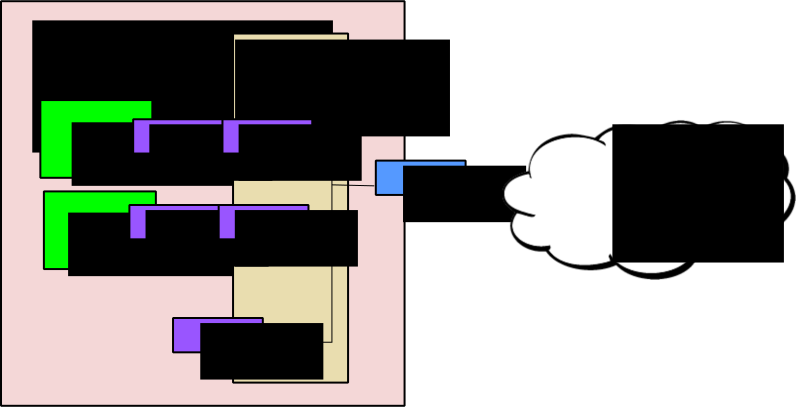
\includegraphics[scale=0.4]{figures/lxc-veth.pdf}
  \label{fig:hpc}
 % \caption{VETH network}
\end{figure}
\end{frame}


\begin{frame}[label=sec-3-3]{Linux kernel version}
32 containers running on: 8,16,32 physical machines.

\begin{columns}
\begin{column}{0.5\textwidth}
\begin{block}{Max performance gain}


\begin{itemize}
\item 3.2 -> 3.16 \textasciitilde{}77\%.
\item 3.16 -> 4.0 \textasciitilde{}11\%.
\end{itemize}
\end{block}
\end{column}

\begin{column}{0.5\textwidth}





\begin{figure}[!h]
  \center
  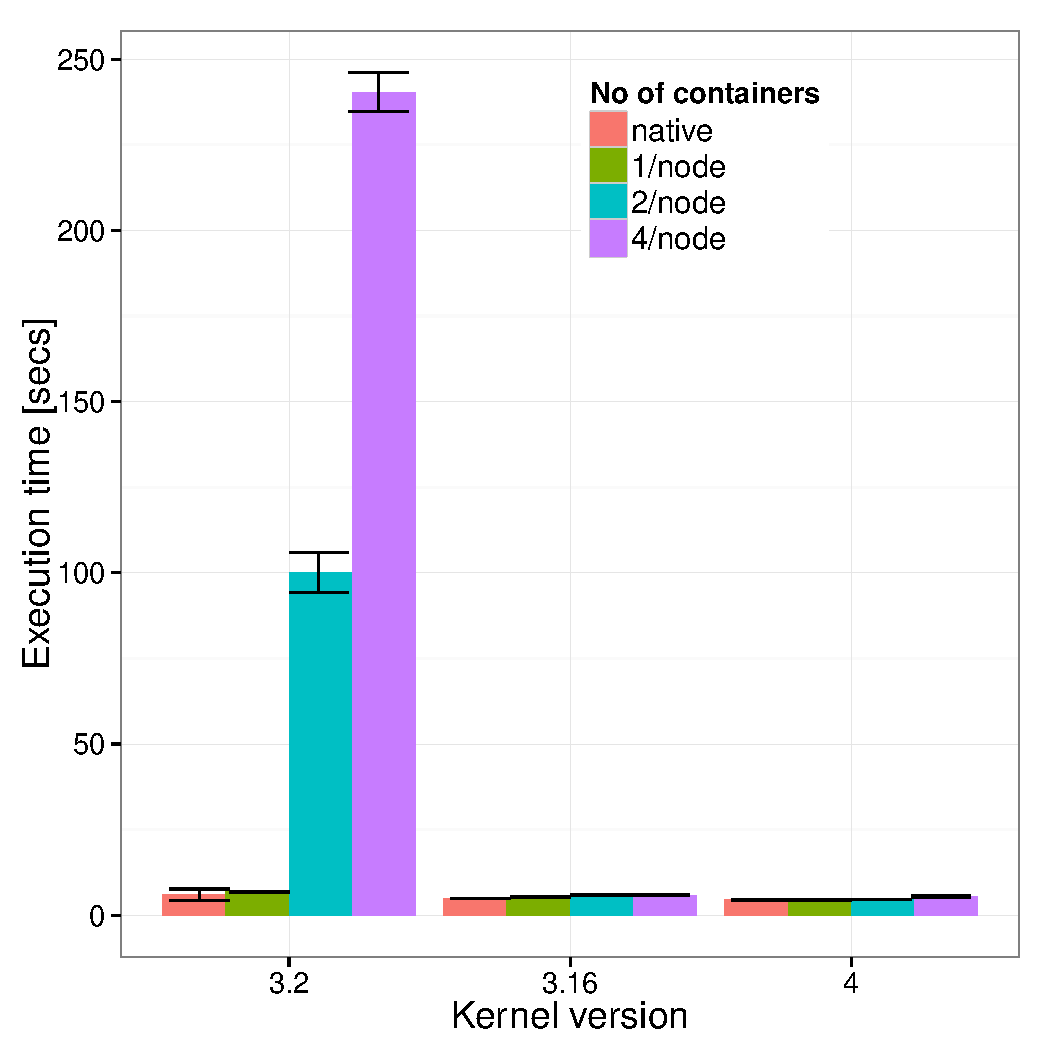
\includegraphics[scale=0.32]{figures/execution_time-kernel-cgB.pdf}
  \label{fig:hpc}
  \caption{CG.B}
\end{figure}
\end{column}
\end{columns}
\end{frame}

\begin{frame}[label=sec-3-4]{Oversubscription}
64 containers running over: 8,16,32,64 physical machines.

\begin{columns}
\begin{column}{0.5\textwidth}
\begin{block}{Results}

\begin{itemize}
\item Using Linux kernel 4.0, there is not significant difference between running 1 or 2 container per physical machine.
\end{itemize}
\end{block}
\end{column}

\begin{column}{0.5\textwidth}


\begin{figure}[!h]
  \center
  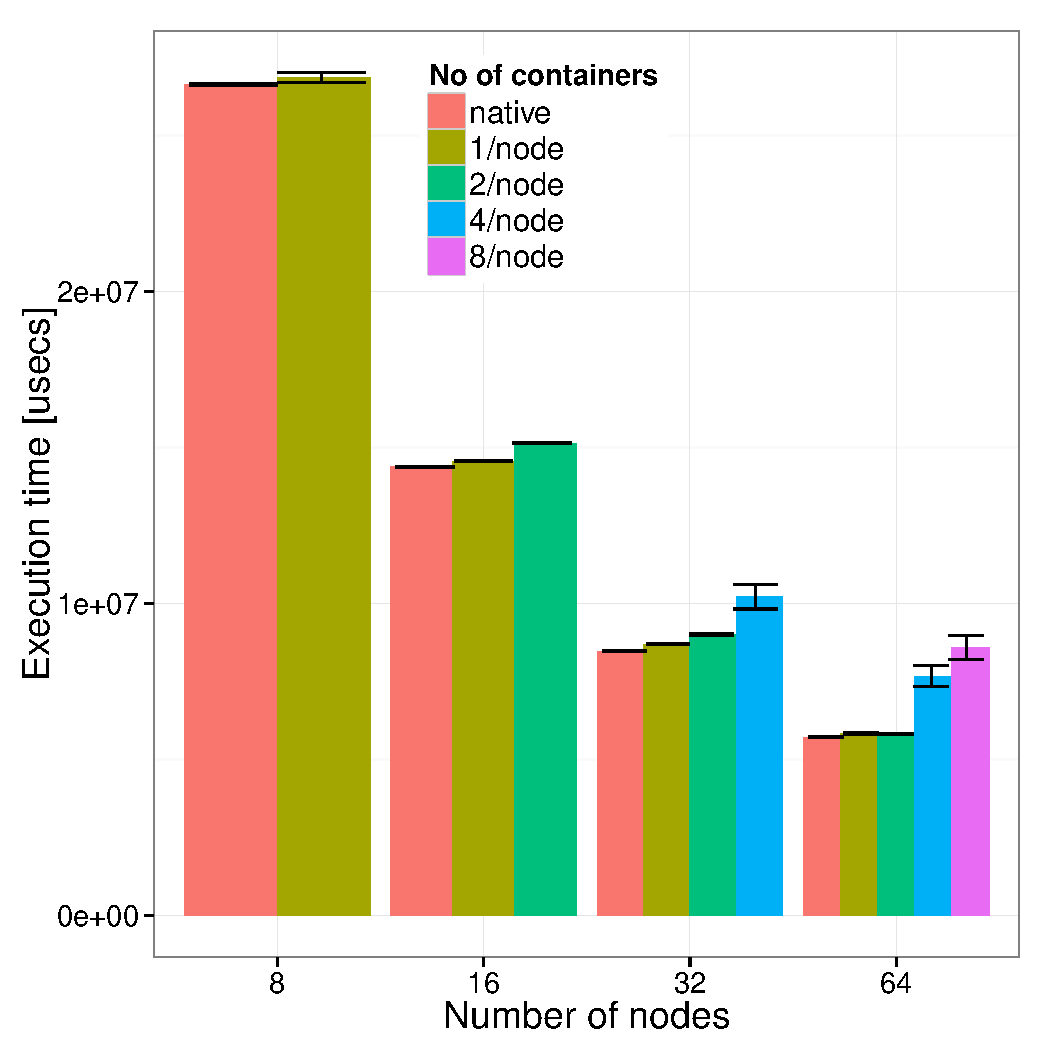
\includegraphics[scale=0.33]{figures/execution_time-tso-40.pdf}
  \label{fig:hpc}
  \caption{LU.B}
\end{figure}
\end{column}
\end{columns}
\end{frame}

\begin{frame}[label=sec-3-5]{Inter-container communication}
\begin{itemize}
\item \emph{container} and \emph{SM}: 1 physical node.
\item \emph{native} : 2, 4, 8 physical nodes.
\end{itemize}

All running the equivalent number of MPI processes.

\begin{figure}[H]
  \centering
\begin{subfigure}[b]{0.42\textwidth}
    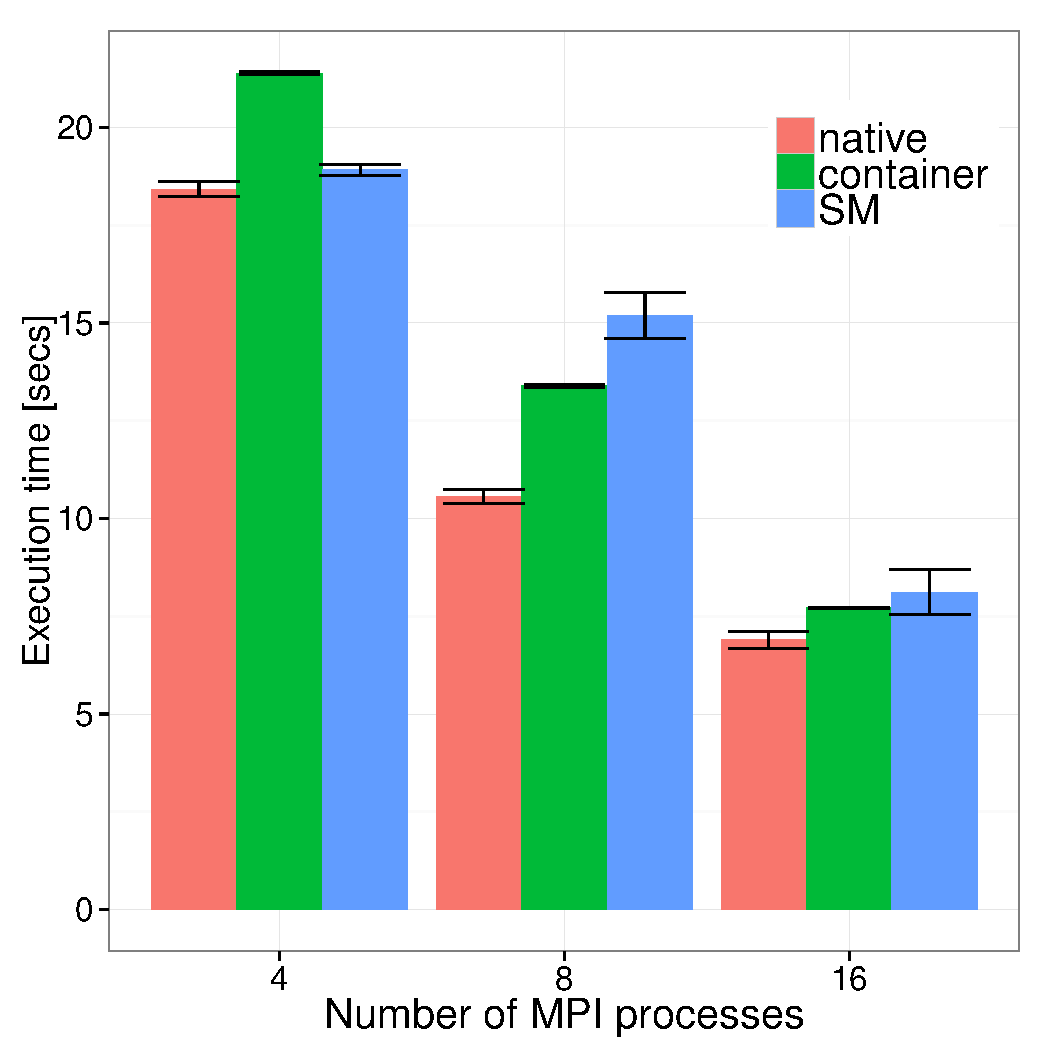
\includegraphics[scale=0.25,angle=0]{figures/inter-container-mgC.pdf}
    \caption{CG Class B}
  \end{subfigure}
  \begin{subfigure}[b]{0.42\textwidth}
    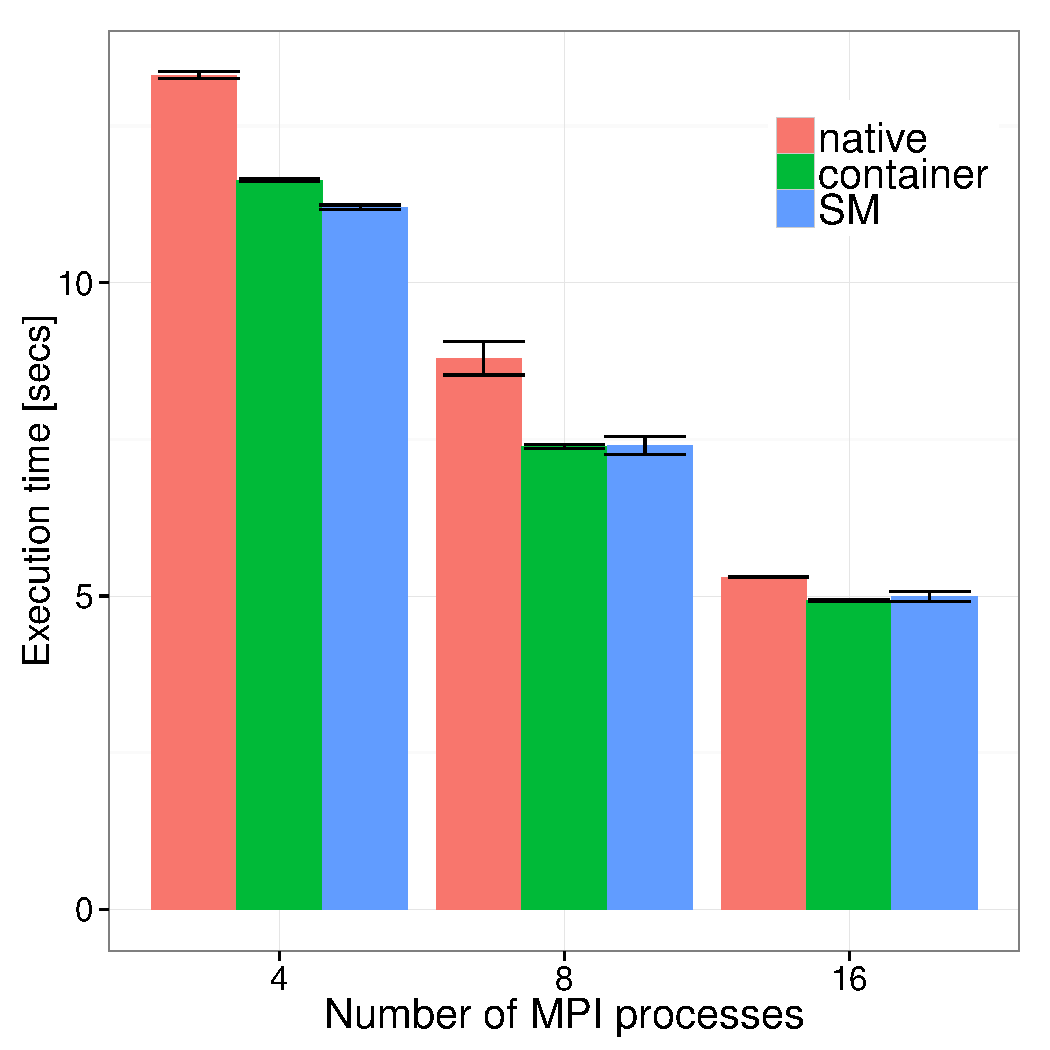
\includegraphics[scale=0.25,angle=0]{figures/inter-container-isC.pdf}
    \caption{IS Class C}
  \end{subfigure}
\end{figure}
\end{frame}

\begin{frame}[label=sec-3-6]{Inter-container communication}
\begin{itemize}
\item Although inter-container communication is faster
than communication among physical machines, there is an important degradation
of the CPU performance for applications that are memory bound.

\item Virtual network device does not add an extra cost.
\end{itemize}
\end{frame}

\begin{frame}[label=sec-3-7]{Multinode inter-container communication}
\begin{itemize}
\item 16 MPI processes were run per physical machine or container
\item We used a maximum of 32 physical machines.
\end{itemize}

\begin{figure}
  \centering
  \begin{subfigure}[b]{0.42\textwidth}
    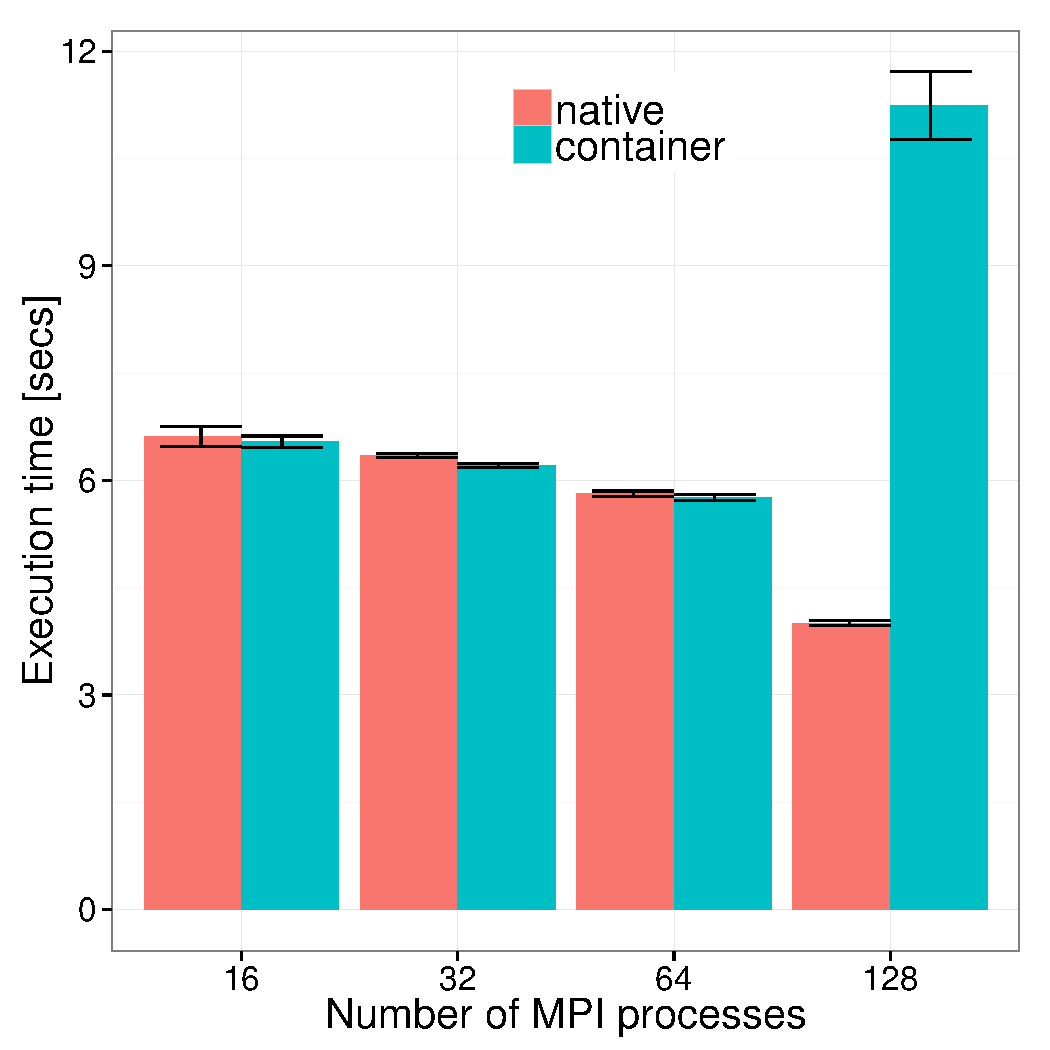
\includegraphics[scale=0.25,angle=0]{figures/veth_overhead-tso-cgB.pdf}
    \caption{CG Class B}
  \end{subfigure}
  \begin{subfigure}[b]{0.42\textwidth}
    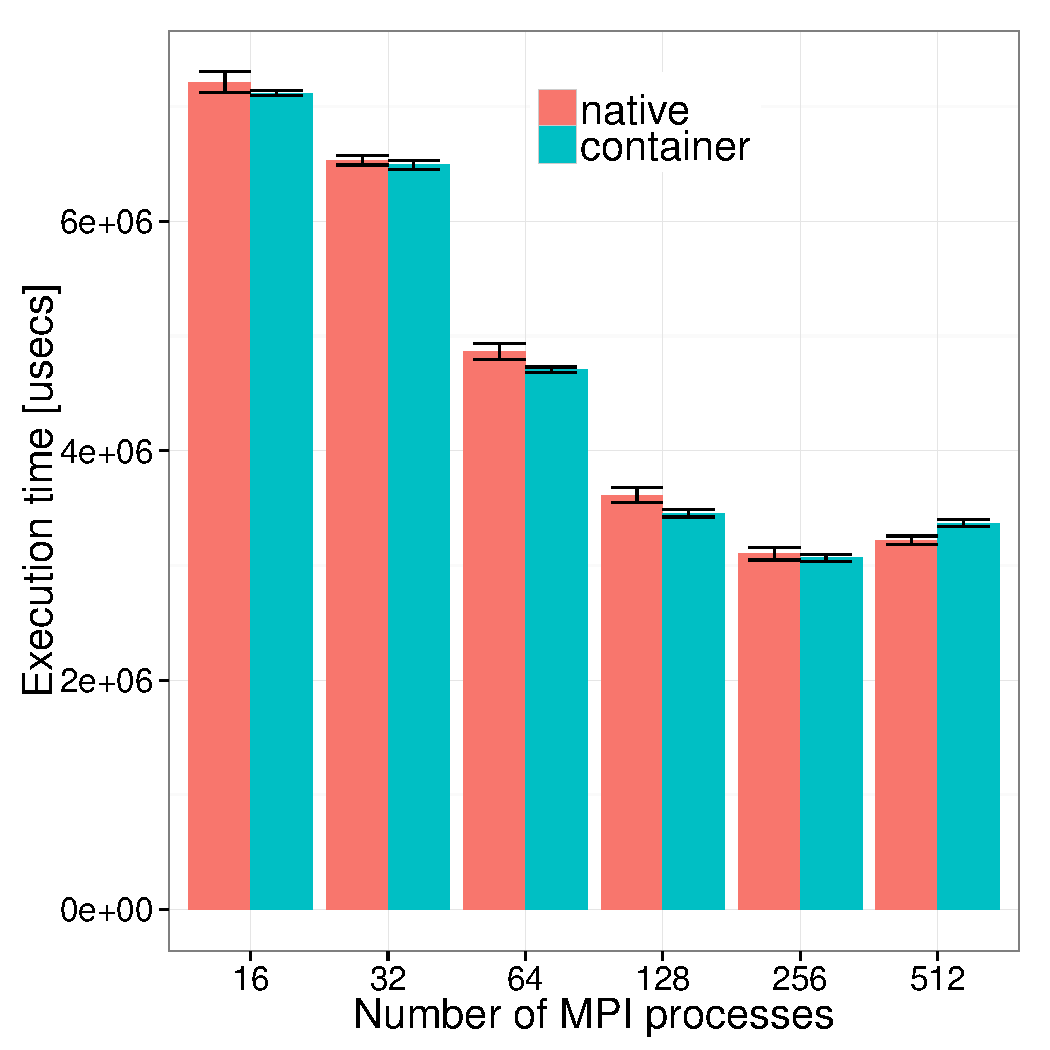
\includegraphics[scale=0.25,angle=0]{figures/veth_overhead-tso-ftB.pdf}
    \caption{FT Class B}
  \end{subfigure}
\end{figure}
\end{frame}

\begin{frame}[label=sec-3-8]{Multinode inter-container communication}
\begin{itemize}
\item Benchmarks with low  MPI communication: we observed a maximum overhead of \alert{5.97\%} (with \alert{512 MPI processes}).
\item Benchmarks with an intensive MPI communication: we observed a higher overhead starting from \alert{30\%} for the benchmark LU.

\item CG reaches \alert{180\%} of overhead when \alert{128} MPI processes are used.
This benchmarks sends a high number of MPI messages, around
a 1000 times more than the first group of benchmarks
which increase network congestion and leads to TCP timeouts.
\end{itemize}
\end{frame}

\begin{frame}[label=sec-3-9]{Multinode inter-container communication}
\begin{itemize}
\item It was shown how network bound applications can be severely affected by
the default container network interconnection.

\item We found a way to alleviate the overhead
by tweaking parameters of the Linux network stack.

\begin{itemize}
\item TCP minimum retransmission timeout (RTO)
\item TCP Selective Acknowledgments (SACK)
\end{itemize}
\end{itemize}
\end{frame}


\section{Conclusions}
\label{sec-4}
\begin{frame}[label=sec-4-1]{In this work \ldots{}}
\begin{itemize}
\item We study the impact of using containers in the context of HPC research.

\item We evaluate two interesting uses of containers in the context of HPC research: portability of complex software stacks
and oversubscription.

\item We carried out the evaluation under a configuration expected to be found in an HPC context.
\end{itemize}
\end{frame}

\begin{frame}[label=sec-4-2]{What did we find?}
\begin{itemize}
\item The limits of using containers.
\item The type of application that are affected the most.
\item The level of oversubscription containers achieved without impacting considerably the application performance.
\item The technology is getting mature and performance issues are being addressed through the constant evolution of the Linux kernel.
\end{itemize}
\end{frame}


\begin{frame}[label=sec-4-3]{Future work}
\begin{itemize}
\item Measure the impact of using containers on disk I/O and other
containers features like memory limitation.

\item The overhead observed could be diminished by integrating
more advance network interconnection such as Linux's \emph{macvlan}, SR-IOV or OpenvSwitch\footnote{http://openvswitch.org/}.
\end{itemize}
\end{frame}

{\setbeamercolor{background canvas}{bg=basicallyblack}
\usebeamercolor[fg]{inverted text}
\begin{frame}[label=sec-4-4]{The end}

\vspace{3cm}
\par {\usebeamerfont{title} {\center Thank you} }\par
\vspace{3cm}\hfill
\end{frame}
}



\section{Bibliography}
\label{sec-5}
\begin{frame}[label=sec-5-1]{Bibliography}

\bibliography{distem_validation.bib}
\bibliographystyle{plain}
\appendix
\end{frame}
% Emacs 24.3.1 (Org mode 8.2.10)
\end{document}
